The purpose of this section is evaluate Algorithm~\ref{alg:priv-hc-hsbm} designed for the HSBM model. First, we outline our methods and then we discuss our results.

\paragraph{Experimental Setup}
We tested our clustering algorithms on a real-world graph and generated synthetic graphs from the HSBM model. We compared the performance of \dphchsbm{} to several baseline algorithms.
We ran algorithms at $\epsilon \in \{0.5, 1.0, 2.0\}$, as well as with no privacy.

To enable the replication of our work, we make the code available {\bf open-source} \footnote{\url{https://bitbucket.org/jjimola/dphc/src/master/}}.

\paragraph{Datasets} Our real-world graph was generated from the MNIST digits dataset~\citep{lecun1998mnist} (with 1797 digits) by, for each digit, adding an undirected edge corresponding to one of its 120 nearest neighbors in pixel space. We generated graphs from $\hsbm(B, P, f)$ with $n=2048$ nodes, $k = \{4, 8\}$ blocks, with block sizes chosen proportional to $\{1, \gamma, \ldots, \gamma^{k-1}\}$, where $\gamma^{k-1} = 3$. This has the effect of creating differently-sized blocks. We selected $P$ to be a balanced tree over the blocks, and $f$ that increases uniformly in the interval $[0.1, 0.9]$ as the tree is descended. 

\paragraph{Algorithms} We ran \dphchsbm{} and several baseline algorithms. In the implementation of \dphchsbm{}, we used a modified version of \dpcom{} for practical considerations. This does not affect the privacy guarantees but it simplifies the algorithm. In particular, we privately release $\tilde{A}_1$ using the Laplace mechanism, and compute $\Pi_{\tilde{A}_1}(\hat{A}_2)$ without projection. We are then able to add Gaussian noise tailored to the sensitivity of $\Pi_{\tilde{A}_1}$, rather than to $\Gamma$ which proved to be a rough upper bound in practice.

For our baselines, we considered a naive private approach in which we release $A$ using the Laplace mechanism and truncate these values to be non-negative to form a sanitized, weighted graph. Then, we ran single, complete, and average linkage, and recorded the best of these methods. We refer collectively to these baselines as \linkage{}. Second, we formed a tree by recursively partitioning the graph into its (approximately) sparsest cut. As shown in~\citet{charikar2017approximate}, this is an $O(\sqrt{\log n}, 0)$-approximation in the \textit{sanitized} graph. We refer to this baseline as \sparsecut{}.

\paragraph{Metrics}
For each graph and clustering algorithm, and the value of $\epsilon$, we computed $\cost_G(T)$, averaged over 5 runs.

\subsection{Results}\label{sec:exp-discuss}
\begin{figure}
    \begin{subfigure}[b]{\linewidth}
            \centering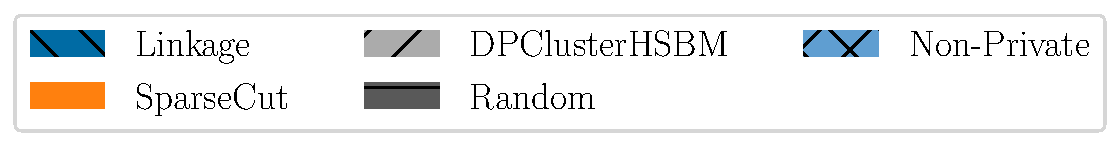
\includegraphics[width=0.8\linewidth]{plots/legend.pdf}
    \end{subfigure}\\
    \begin{subfigure}[b]{\linewidth}
        \centering
        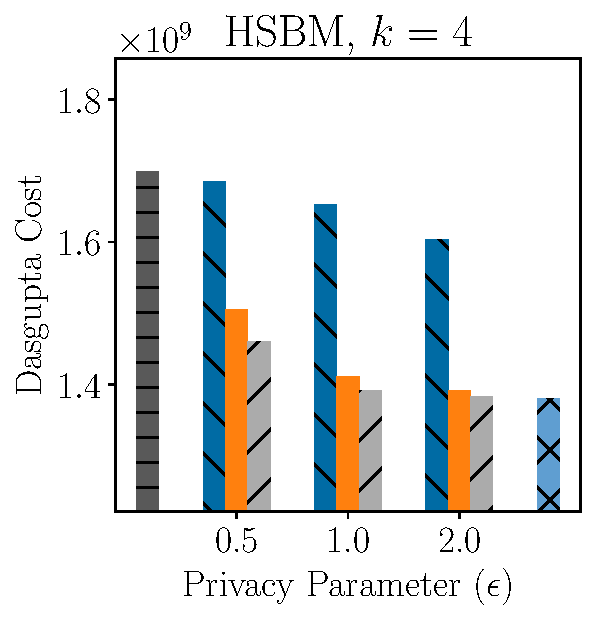
\includegraphics[width=0.48\linewidth]{plots/syn_2048_4_cost.pdf}
        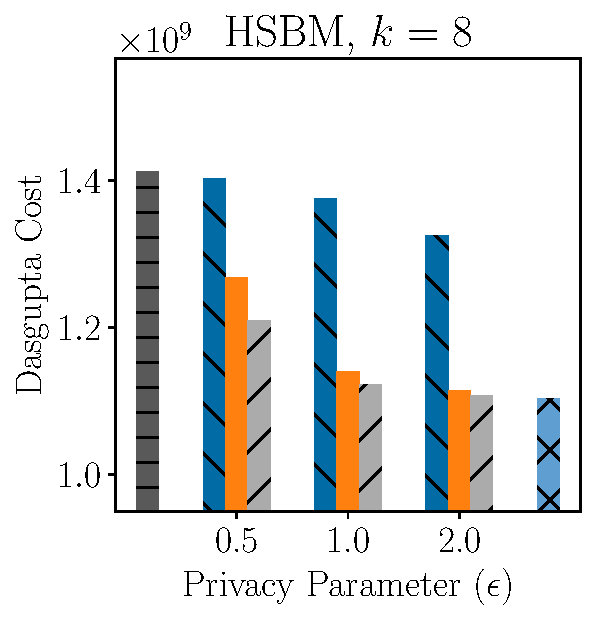
\includegraphics[width=0.48\linewidth]{plots/syn_2048_8_cost.pdf}
        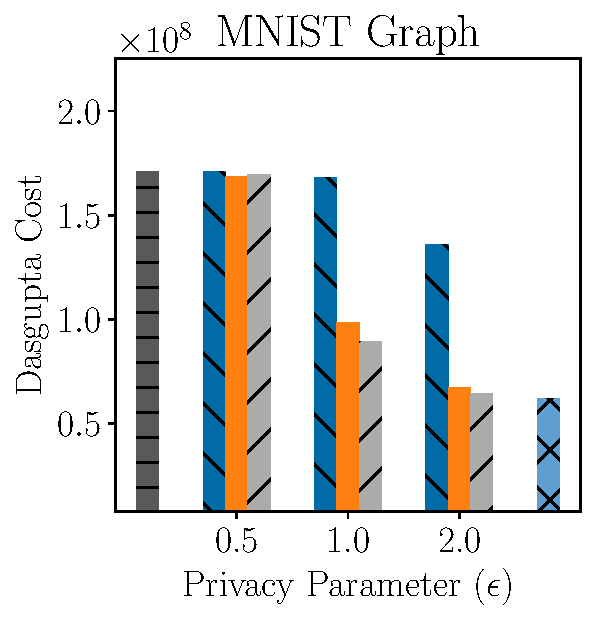
\includegraphics[width=0.48\linewidth]{plots/mnist_cost.pdf}
    \end{subfigure}
    \caption{Cost for HSBM graphs with $2048$ nodes and $k$ clusters and MNIST graph with $1797$ nodes.}
    \label{fig:exp-results}
    
\end{figure}

Our results appear in Figure~\ref{fig:exp-results}. In addition to the cost for each algorithm, we included the cost of a random tree. The data had low variance: for each of the 5 runs used to compute each bar, the values were within $0.5\%$ of each other.

For all trials, 
the cost of \linkage{} was much higher than the other two algorithms; even with $\epsilon = 2$, \linkage{} did not offer improvement of more than $10\%$ reduction in cost over the random tree. Thus, the rest of our discussion focuses on \dphchsbm{} and \sparsecut{}.

For the synthetic graphs,
the cost of \dphchsbm{} is lower than \sparsecut{}, particularly when $\epsilon = 0.5$. In this case, when $k=4$ (resp. $8$), \dphchsbm{} offered a $14.4\%$ (resp. $14.2\%$) reduction in cost over the random tree, whereas \sparsecut{} offered an $11.5\%$ (resp. $10.3\%$) reduction.
Thus, \dphchsbm{} offers up to $38\%$ more reduction in cost than \sparsecut{}, over the cost of a random tree. Even when $\epsilon = 0.5$, the cost of \dphchsbm{} is just $5.8\%$ (resp. $9.6\%$) higher than the cost of the best tree with no privacy.

For $\epsilon = 1,2$ on HSBM graphs, the costs of \sparsecut{} and \dphchsbm{} fall to within $1\%$ of each other, though $\dphchsbm{}$ consistently outperforms the former for all values of $\epsilon$. Moreover, notice that for $\epsilon = 2$, the costs of both algorithms are within $1\%$ of the non-private tree, indicating that for higher $\epsilon$ the cost of privacy becomes negligible.

For the graph generated from MNIST, all algorithms perform as poorly as a random tree for $\epsilon = 0.5$. This indicates that the noise introduced by the high privacy constraint destroys the clusters, which are less-well structured than those of the HSBM graphs. At $\epsilon = 1$, the error of \sparsecut{} is $10\%$ higher than \dphchsbm{}. For $\epsilon = 2$, the cost of \sparsecut{} is $5\%$ higher than that of \dphchsbm{}, and \dphchsbm{} attains error within $3\%$ of the best tree with no privacy. This is consistent with our previous observation that \dphchsbm{} offers improvement over the baselines, particularly when $\epsilon$ is not too high.

\section{Conclusion}
We have considered hierarchical clustering under differential privacy in Dasgupta's cost framework. While strong lower bounds exist for the problem, we have proposed algorithms with nearly matching approximation guarantees. Furthermore, we showed the lower bounds can be overcome in the HSBM, and nearly optimal trees can be found in this setting using efficient methods. For future work, one could consider private hierarchical clustering in a less structured model than the HSBM in hopes of overcoming the lower bound here as well.